\documentclass[tikz,border=0pt,multi]{standalone}
\usepackage[utf8]{inputenc}
\usepackage{graphicx}
\usepackage[export]{adjustbox}
% \usepackage{times}
\usepackage{tikz}
\renewcommand{\familydefault}{\sfdefault}
\usepackage[T1]{fontenc}
\usepackage{uarial}
\usetikzlibrary{fit,backgrounds,shapes,positioning,arrows,arrows.meta}

\begin{document}
\pgfdeclarelayer{main}
\pgfdeclarelayer{z1}
\pgfdeclarelayer{z2}
\pgfdeclarelayer{z3}
\pgfsetlayers{main,z1,z2,z3}
\begin{tikzpicture}[every node/.style={inner sep=0,outer sep=0}]
  \tikzstyle{arr}=[-{Latex[scale=0.65]}];
  \coordinate (A) at (0,0);
  \node (fig1) {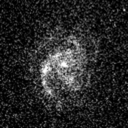
\includegraphics[width=17pt]{imgs/F378.png}};
  \node [yshift=-9pt] (fig2) at (fig1.south) {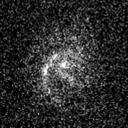
\includegraphics[width=17pt]{imgs/F395.png}};
  \node [yshift=-9pt] (fig3) at (fig2.south) {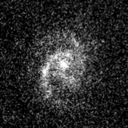
\includegraphics[width=17pt]{imgs/F410.png}};
  \node [yshift=-9pt] (fig4) at (fig3.south) {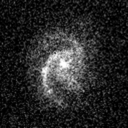
\includegraphics[width=17pt]{imgs/F430.png}};

  \node [xshift=9pt] (fig5) at (fig1.east){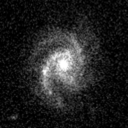
\includegraphics[width=17pt]{imgs/F515.png}};
  \node [yshift=-9pt] (fig6) at (fig5.south) {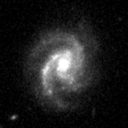
\includegraphics[width=17pt]{imgs/F660.png}};
  \node [yshift=-9pt] (fig7) at (fig6.south) {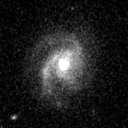
\includegraphics[width=17pt]{imgs/F861.png}};
  \node [yshift=-9pt] (fig8) at (fig7.south){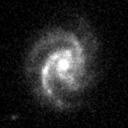
\includegraphics[width=17pt]{imgs/G.png}};

  \node [xshift=9pt] (fig11) at (fig5.east) {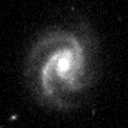
\includegraphics[width=17pt]{imgs/I.png}};
  \node [yshift=-9pt] (fig12) at (fig11.south) {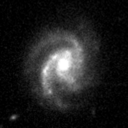
\includegraphics[width=17pt]{imgs/R.png}};
  \node [yshift=-9pt] (fig13) at (fig12.south) {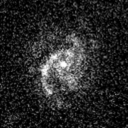
\includegraphics[width=17pt]{imgs/U.png}};
  \node [yshift=-9pt] (fig14) at (fig13.south) {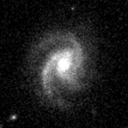
\includegraphics[width=17pt]{imgs/Z.png}};


  \node (figcolor) at (fig12.south) [xshift=44pt] {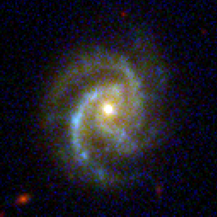
\includegraphics[width=52pt]{imgs/color.png}};
  \path[arr] (fig11.north east) edge[] (figcolor.north west);
  \path[arr] (fig14.south east) edge[] (figcolor.south west);

  \node[right of=figcolor,xshift=38pt,yshift=27pt,draw,inner sep=2pt,minimum width=56pt,align=center] (member1) {\scriptsize{Classificador I} \\[-6pt]\tiny{InceptionResnetV2}};
  \node[right of=figcolor,xshift=38pt,yshift=9pt,draw,inner sep=2pt,minimum width=56pt,align=center] (member2) {\scriptsize{Classificador II} \\[-6pt]\tiny{EfficientNetB2}};
  \node[right of=figcolor,xshift=38pt,yshift=-9pt,draw,inner sep=2pt,minimum width=56pt,align=center] (member3) {\scriptsize{Classificador III} \\[-6pt]\tiny{DenseNet-169}};
  \node[right of=figcolor,xshift=38pt,yshift=-27pt,draw,inner sep=2pt,minimum width=56pt,align=center] (member4) {\scriptsize{Classificador IV} \\[-6pt]\tiny{DenseNet-201}};


  \draw[arr] (figcolor) -- (member1.west);
  \draw[arr] (figcolor) -- (member2.west);
  \draw[arr] (figcolor) -- (member3.west);
  \draw[arr] (figcolor) -- (member4.west);


  \node[xshift=97pt,yshift=-3pt] (prob1) at (figcolor.east) {\tiny{\{P(E); P(S)\}}};
  \node[yshift=5pt] (prob2) at (prob1.north) {\tiny{\{P(E); P(S)\}}};
  \node[yshift=5pt] (prob3) at (prob2.north) {\tiny{\{P(E); P(S)\}}};
  \node[yshift=-5pt] (prob4) at (prob1.south) {\tiny{\{P(E); P(S)\}}};
  \node[draw,thin,inner sep=3pt,fit=(prob3.north) (prob4.south) (prob1.east) (prob1.west),dash pattern={on 1pt off 1.5pt}] (probbox) {};


  \draw[arr] (member1.east) -- (probbox);
  \draw[arr] (member2.east) -- (probbox);
  \draw[arr] (member3.east) -- (probbox);
  \draw[arr] (member4.east) -- (probbox);


  \node[draw,thin,inner sep=4pt,rotate=90,yshift=-16pt,minimum width=64pt] (logistic) at (probbox.east) {\scriptsize{Meta-Modelo}};
  \path[arr] (probbox.east) edge (logistic.north);


  \node[xshift=13pt,yshift=14pt,outer sep=1pt] (pE) at (logistic.south) {\tiny{P(E)}};
  \node[xshift=13pt,yshift=-14pt,outer sep=1pt] (pS) at (logistic.south) {\tiny{P(S)}};
  \path[arr] (logistic) edge (pE.west);
  \path[arr] (logistic) edge (pS.west);
\end{tikzpicture}
\end{document}